\documentclass[12pt]{scrartcl}
\usepackage{numprint}
\usepackage{enumerate}
\usepackage{fontspec}
\usepackage{amsmath}
\usepackage{amssymb}
\usepackage{minted}
\usepackage{graphicx}
\usepackage{float}
\usepackage[math-style = upright]{unicode-math}
\usepackage[final=true,step=1]{microtype}
%\SetTracking{encod@ing={*}, shape=sc}{40}

\setminted{breaklines=true,autogobble=true,bgcolor=lightgray!15!white}
\setsansfont[BoldFont=Fira Sans Medium]{Fira Sans Light}
\setmonofont[BoldFont=JetBrains Mono Regular]{JetBrains Mono Light}
\setmathfont{TeX Gyre Pagella Math}
\setmainfont{TeX Gyre Pagella}
\usepackage[french]{babel}
\title{Quelques activités de NSI en lien avec la cybersécurité}
\author{\textsf{Formateurs NSI Rennes}}
\date{\textsf{mai 2023}}

\begin{document}
\maketitle

\begin{abstract}
    Ceci est une ébauche de travail basée sur ce que nous avons fait le lundi 22 mars.
    Dans la perspective des formations à dispenser, peut-être faut-il se contraindre à montrer que les contenus proposés s'intègrent dans le programme sans le surcharger et expliquer autant que possible la plus-value qu'elles peuvent apporter.\\
    Lors de ces formations, il faudrait également pouvoir mettre les collègues en situation élève pour qu'ils découvrent une activité en la pratiquant : cela les implique davantage et démontre qu'elle est parfaitement faisable et, espérons-le, intéressante.
\end{abstract}

\section{Considérations générales}

%L'omniprésence de la cybersécurité et de la cyberdéfense n'est plus à démontrer, qu'elle s'adresse aux particuliers, aux administrations ou aux entreprises.\\

Nous proposons ici des activités qui
\begin{itemize}
    \item entrent dans le cadre du programme officiel, de sorte qu'elles peuvent être menées sans empiéter sur les temps de cours ;
    \item adoptent un positionnement raisonnable en terme d'équilibre culture / technique : d'une part, il ne faut pas revoir une notion déjà étudiée par le passé à moins d'y ajouter quelque chose d'essentiel, d'autre part les notions rencontrées peuvent être intimidantes du point de vue technique ou mathématique, on essaie donc de s'en abstraire sans dénaturer l'activité.
\end{itemize}

\section{Observation contextualisée d'une fonction de hachage}

\textbf{But : } Faire constater aux élèves ce qui est effectivement transmis au serveur lors de la validation d'un formulaire comportant des données sensibles.

\textbf{Lien avec le cours : } Complètement en phase avec le volet IHM de première.

\textbf{Partie technique : } Du HTML et du Javascript, très simple, une fonction de hachage est exposée \textit{pour s'en servir}.\\

Un travail d'observation des fonctions de hachage peut être fait avec la librairie standard de Python.


\begin{figure}[H]
    \begin{minted}[fontsize=\scriptsize,breaklines=true]{javascript}
function validateForm() {
    // On récupère la valeur de "fPassword"
    let x = document.forms["myForm"]["fPassword"].value; 

    // si cette valeur correspond bien au motif désiré (voir plus bas)
    if (x.match("^(?=.*[a-z])(?=.*[A-Z])(?=.*[0-9])(?=.*[ -/:-@\[-`{-~]).{8,16}$") == null){
        alert("Le mot de passe doit contenir une minuscule, une majuscule, un chiffre,
        un caractère spécial et comporter entre 8 et 16 caractères.");
        
        // On vide le champ fPassword
        document.forms["myForm"]["fPassword"].value = ""; 
        return false;
    }

    // Si le mot de passe est valable, on ne l'envoie pas, on envoie son hash...
    document.forms["myForm"]["fPassword"].value = SHA256(x); 
}
\end{minted}
    \caption{code Javascript de la fonction de validation du formulaire}
\end{figure}

Le code de la fonction SHA256 figure après le code ci-dessus, pour observation par l'élève.


\begin{figure}[H]
    \begin{center}
        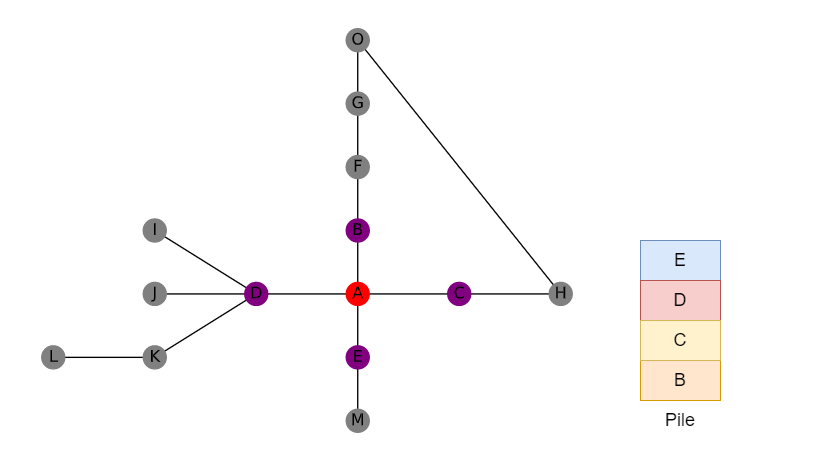
\includegraphics[width=5cm]{img/01.png}
    \end{center}
    \caption{validation du formulaire}
\end{figure}

\begin{figure}[H]
    \begin{center}
        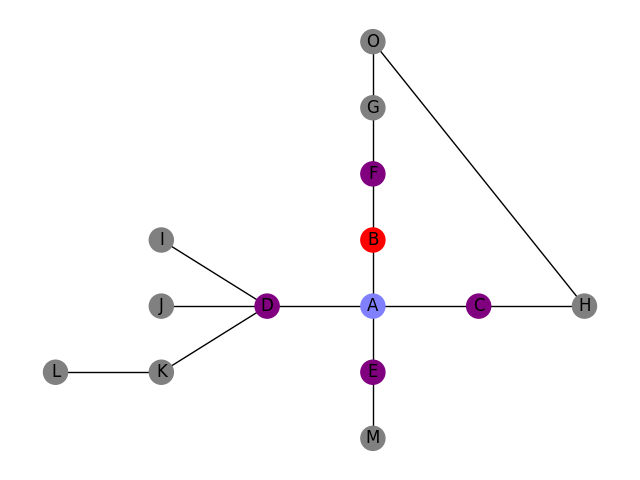
\includegraphics[width=\linewidth]{img/02.png}
    \end{center}
    \caption{observation des données transmises \textit{via} la méthode \texttt{GET}}
\end{figure}

\section{Faire  «  comme HTTPS  »  }
\textbf{But :} Faire connaître et utiliser les algorithmes de chiffrements.

\textbf{Lien avec le cours :} On fait comme le protocole HTTPS : une donnée est encryptées avec AES (encryptage symétrique), la clé de cryptage est encodée en RSA.

\textbf{Partie technique :}
\begin{itemize}
    \item utilisation de bibliothèques de cryptographie ;
    \item on peut expliquer les algorithmes \textit{sans les prouver} ;
    \item les élèves peuvent créer une petite Interface graphique.
\end{itemize}


\begin{figure}[H]
    \begin{center}
        \includegraphics[width=5cm]{img/seQre.png}
    \end{center}
    \caption{interface minimaliste créée avec \texttt{flet}.}
\end{figure}

\section{L'attaque de l'homme du milieu en débranché}

Diffie Hellman avec des confettis ? Des paillettes ? Du sable ?

Diffie Hellman + homme du milieu

AES + homme du milieu
RSA + homme du milieu 



\section{En plan}
\begin{itemize}
    \item Travail en première sur les critères de sécurité d'un mot de passe.
    \item Est-ce que c'est possible de faire un fil rouge ?
    \item Explorer autour des cookies.
    \item l'homme du milieu.
    \item les certificats ?
\end{itemize}
RGS pour cookies

PSSI pour se former (long)

Chiffrer ou certifier est la réponse à l'homme du milieu ?

Man in the middle en débranché ?

\end{document}